% This is "sig-alternate.tex" V2.0 May 2012
% This file should be compiled with V2.5 of "sig-alternate.cls" May 2012
%
% This example file demonstrates the use of the 'sig-alternate.cls'
% V2.5 LaTeX2e document class file. It is for those submitting
% articles to ACM Conference Proceedings WHO DO NOT WISH TO
% STRICTLY ADHERE TO THE SIGS (PUBS-BOARD-ENDORSED) STYLE.
% The 'sig-alternate.cls' file will produce a similar-looking,
% albeit, 'tighter' paper resulting in, invariably, fewer pages.
%
% ----------------------------------------------------------------------------------------------------------------
% This .tex file (and associated .cls V2.5) produces:
%       1) The Permission Statement
%       2) The Conference (location) Info information
%       3) The Copyright Line with ACM data
%       4) NO page numbers
%
% as against the acm_proc_article-sp.cls file which
% DOES NOT produce 1) thru' 3) above.
%
% Using 'sig-alternate.cls' you have control, however, from within
% the source .tex file, over both the CopyrightYear
% (defaulted to 200X) and the ACM Copyright Data
% (defaulted to X-XXXXX-XX-X/XX/XX).
% e.g.
% \CopyrightYear{2007} will cause 2007 to appear in the copyright line.
% \crdata{0-12345-67-8/90/12} will cause 0-12345-67-8/90/12 to appear in the copyright line.
%
% ---------------------------------------------------------------------------------------------------------------
% This .tex source is an example which *does* use
% the .bib file (from which the .bbl file % is produced).
% REMEMBER HOWEVER: After having produced the .bbl file,
% and prior to final submission, you *NEED* to 'insert'
% your .bbl file into your source .tex file so as to provide
% ONE 'self-contained' source file.
%
% ================= IF YOU HAVE QUESTIONS =======================
% Questions regarding the SIGS styles, SIGS policies and
% procedures, Conferences etc. should be sent to
% Adrienne Griscti (griscti@acm.org)
%
% Technical questions _only_ to
% Gerald Murray (murray@hq.acm.org)
% ===============================================================
%
% For tracking purposes - this is V2.0 - May 2012

\documentclass{sig-alternate-2013}

\begin{document}
%
% --- Author Metadata here ---
\conferenceinfo{ACM International Conference on Information and Knowledge Management}{'14 Shanghai, China}
%\CopyrightYear{2007} % Allows default copyright year (20XX) to be over-ridden - IF NEED BE.
%\crdata{0-12345-67-8/90/01}  % Allows default copyright data (0-89791-88-6/97/05) to be over-ridden - IF NEED BE.
% --- End of Author Metadata ---

\title{A cross benchmark comparison of Learning to Rank methods}
%
% You need the command \numberofauthors to handle the 'placement
% and alignment' of the authors beneath the title.
%
% For aesthetic reasons, we recommend 'three authors at a time'
% i.e. three 'name/affiliation blocks' be placed beneath the title.
%
% NOTE: You are NOT restricted in how many 'rows' of
% "name/affiliations" may appear. We just ask that you restrict
% the number of 'columns' to three.
%
% Because of the available 'opening page real-estate'
% we ask you to refrain from putting more than six authors
% (two rows with three columns) beneath the article title.
% More than six makes the first-page appear very cluttered indeed.
%
% Use the \alignauthor commands to handle the names
% and affiliations for an 'aesthetic maximum' of six authors.
% Add names, affiliations, addresses for
% the seventh etc. author(s) as the argument for the
% \additionalauthors command.
% These 'additional authors' will be output/set for you
% without further effort on your part as the last section in
% the body of your article BEFORE References or any Appendices.

\numberofauthors{3} %  in this sample file, there are a *total*
% of EIGHT authors. SIX appear on the 'first-page' (for formatting
% reasons) and the remaining two appear in the \additionalauthors section.
%
\author{
% You can go ahead and credit any number of authors here,
% e.g. one 'row of three' or two rows (consisting of one row of three
% and a second row of one, two or three).
%
% The command \alignauthor (no curly braces needed) should
% precede each author name, affiliation/snail-mail address and
% e-mail address. Additionally, tag each line of
% affiliation/address with \affaddr, and tag the
% e-mail address with \email.
%
% 1st. author
\alignauthor
Niek Tax\titlenote{affiliated with University of Twente, but written during his time at Avanade Netherlands B.V.}\\
       \affaddr{Avanade Netherlands B.V.}\\
       \affaddr{Versterkerstraat 6}\\
       \affaddr{1322 AP Almere}\\
       \affaddr{The Netherlands}
       \email{niek.tax@avanade.com}
% 2nd. author
\alignauthor
Djoerd Hiemstra\\
       \affaddr{University of Twente}\\
       \affaddr{P.O. Box 217}\\
       \affaddr{7500 AE Enschede}\\
       \affaddr{The Netherlands}
       \email{d.hiemstra@utwente.nl}
% 3rd. author
\alignauthor
Sander Bockting\\
       \affaddr{Avanade Netherlands B.V.}\\
       \affaddr{Versterkerstraat 6}\\
       \affaddr{1322 AP Almere}\\
       \affaddr{The Netherlands}
       \email{sander.bockting@avanade.com}
}

\maketitle
\begin{abstract}

\end{abstract}

% A category with the (minimum) three required fields
\category{H.4}{Information Systems Applications}{Miscellaneous}
%A category including the fourth, optional field follows...
\category{D.2.8}{Software Engineering}{Metrics}[complexity measures, performance measures]

\terms{}

\keywords{, }

\section{Introduction}


\section{The {\secit Body} of The Paper}


\subsection{Type Changes and {\subsecit Special} Characters}
\label{chap:cross_comparison}
As we have seen in Chapter~\ref{chap:benchmark_results}, the evaluation of Learning-to-Rank methods is spread over several benchmark datasets. However, as the Learning-to-Rank methods evaluated differs between benchmarks, no single benchmark comparison can be regarded as a conclusive argument on which Learning-to-Rank method is most accurate.\\

Several studies make a small start in considering Learning-to-Rank methods performance over multiple benchmark datasets. Gomes et al. \cite{Gomes2013} analysed ranking accuracy of a set of models on both LETOR 3.0 and LETOR 4.0. Busa-Fekete et al. \cite{Busa-Fekete2013} compared the accuracy of a small set of models over the LETOR 4.0 datasets, both MSLR datasets, both Yahoo! Learning to Rank Challenge datasets and the OHSUMED dataset from LETOR 3.0. To my knowledge, no structured meta-analysis on ranking accuracy has been conducted where evaluation results on several benchmark collections are taken into account. With a meta-analysis we will compare the performance of Learning-to-Rank methods across the Learning-to-Rank benchmark datasets described in foregoing sections.

\section{Collecting Evaluation Results}
\label{sec:collecting_evaluation_results}
With a literature review we will collect evaluation results on the datasets/collections. The following list presents an overview of the benchmark collections taken into account in the meta-analysis:
\begin{itemize}\itemsep0em
\item LETOR 2.0
\item LETOR 3.0
\item LETOR 4.0
\item Yahoo! Learning to Rank Challenge
\item Yandex Internet Mathematics Competition 2009
\item MSLR-web10/30k
\item WCL2R
\item AOL
\end{itemize}

For the LETOR collections, the evaluation results of the baseline models will be used from LETOR 2.0\footnote{http://research.microsoft.com/en-us/um/beijing/projects/letor/letor2.0/baseline.aspx}, LETOR 3.0\footnote{http://research.microsoft.com/en-us/um/beijing/projects/letor/letor3baseline.aspx} and LETOR 4.0\footnote{http://research.microsoft.com/en-us/um/beijing/projects/letor/letor4baseline.aspx} as listed on the LETOR website.\\

LETOR 1.0, LETOR 3.0, Yahoo! Learning to Rank Challenge, WCL2R and AOL have accompanying papers which were published together with these benchmark collections. Users of those benchmark collections are encouraged to cite these papers. Therefore, we collect evaluation measurements of Learning-to-Rank methods on these benchmark collections through forward literature search. Table~\ref{tbl:ltr_benchmark_forref} presents an overview of the results of this forward literature search. Google Scholar will be used to perform the forward reference search.

\begin{table}[!h]
\begin{tabular}{l|l|l}
Benchmark & Paper & \# of forward references \\
\hline
LETOR 1.0 \& 2.0 & Liu et al. \cite{Liu2007b} & 307\\
LETOR 3.0 & Qin et al. \cite{Qin2010} & 105\\
Yahoo! Learning to Rank Challenge & Chapelle et al. \cite{Chapelle2011a} & 102\\
AOL dataset & Pass et al. \cite{Pass2006} & 339\\
WCL2R & Alc{\^a}ntara et al. \cite{Alcantara2010} & 2\\
\end{tabular}
\caption{Forward references of Learning-to-Rank benchmark papers}
\label{tbl:ltr_benchmark_forref}
\end{table}

The LETOR 4.0, MSLR-web10/30k and Yandex Internet Mathematics Competition 2009 benchmark collections were not accompanied with a describing study. To collect measurements of Learning-to-Rank methods evaluated on these benchmarks, a Google Scholar search is performed on the name of the benchmark. Table~\ref{chap:benchmark_results} shows the results of this literature search.

\begin{table}[!h]
\begin{tabular}{l|l}
Benchmark & Google scholar search results \\
\hline
LETOR 4.0 & 75 results \\
MSLR-web10k & 16 results \\
MSLR-web30k & 15 results \\
Yandex Internet Mathematics Competition & 1 result \\ 
\end{tabular}
\caption{Google scholar search results for Learning-to-Rank benchmarks}
\label{tbl:ltr_benchmark_searchres}
\end{table}

\section{Comparison Methodology}
The LETOR 3.0 paper \cite{Qin2010} states that it may differ between datasets what the most accurate ranking methods are. To evaluate the overall performance of Learning-to-Rank methods over the multiple datasets in the LETOR 3.0 collections, Qin et al. \cite{Qin2010} proposed a measure called \emph{winning number} as the number of other algorithms that an algorithm can beat over the set of datasets. Formally the winning number measure is defined as\\

$\text{Winning Number}_i(M) = \sum\nolimits_{j=1}^n \sum\nolimits_{k=1}^m I_{\{M_i(j)>M_k(j)\}}$\\

where $j$ is the index of a dataset, $n$ the number of datasets in the comparison, $i$ and $k$ are indices of an algorithm, $M_i(j)$ is the performance of the $i$-th algorithm on the $j$-th dataset, $M$ is a ranking measure (such as NDCG or MAP), and $I_{\{M_i(j)>M_k(j)\}}$ is an indicator function such that\\

$I_{\{M_i(j)>M_k(j)\}} = \begin{cases}
1 & \text{if } M_i(j) > M_k(j), \\
0 & \text{otherwise}
\end{cases}$\\

In contrast to the winning number comparison on LETOR 3.0, there will not be accuracy measurements for each algorithm on each dataset in our meta-analysis. To compare algorithms based on a sparse set of evaluation measurements, a normalised version of the Winning Number metric will be used. This Normalised Winning Number takes only those datasets into account that an algorithm is evaluated on and divides this by the theoretically highest Winning Number that an algorithm would have had in case it it would have been the most accurate algorithm on all datasets on which it has been evaluated. We will redefine the indicator function $I$ in order to only take into account those datasets that an algorithm is evaluated on, as \\

$I_{\{M_i(j)>M_k(j)\}} = \begin{cases}
1 & \text{if } M_i(j) \text{ and } M_k(j) \text{ are both defined and } M_i(j) > M_k(j), \\
0 & \text{otherwise}
\end{cases}$\\

From now on this adjusted version of Winning Number will be references to as \emph{Normalised Winning Number}. The mathematical definition of Normalised Winning Number is\\

$\text{Normalised Winning Number}_i(M) = \frac{\text{Winning Number}_i(M)}{\text{Ideal Winning Number}_i(M)}$\\

\noindent
where Ideal Winning Number is defined as\\

$\text{Ideal Winning Number}_i(M) = \sum\nolimits_{j=1}^n \sum\nolimits_{k=1}^m D_{\{M_i(j),M_k(j)\}}$\\

where $j$ is the index of a dataset, $n$ the number of datasets in the comparison, $i$ and $k$ are indices of an algorithm, $M_i(j)$ is the performance of the $i$-th algorithm on the $j$-th dataset, $M$ is a ranking measure (such as NDCG or MAP), and $D_{\{M_i(j),M_k(j)\}}$ is an evaluation definition function such that\\

$D_{\{M_i(j),M_k(j)\}} = \begin{cases}
1 & \text{if } M_i(j) \text{ and } M_k(j) \text{ are both defined}, \\
0 & \text{otherwise}
\end{cases}$\\

NDCG@3, NDCG@5, NDCG@10 and MAP are chosen as metrics on which the meta-analysis will be performed. These metrics seem to be the most frequently used evaluation metrics in most of the used benchmark datasets. An exception is the Yahoo! Learning to Rank Challenge datasets on which mainly ERR is used as main evaluation metric. The lack of use of the ERR metric in other benchmarks makes it unsuitable for a cross-benchmark comparison. By making the decision to include NDCG at three cut-off points and only a single MAP entry, we implicitly attain a higher weight for NDCG compared to MAP on an analysis that combines all measurements on the four metrics. This implicit weighting is arbitrary and therefore undesirable, but the number of algorithm evaluation results gained by this makes it a pragmatic approach.

\section{Evaluation Results Found in Literature}
Table \ref{tab:ltr_methods_used} gives an overview of the Learning-to-Rank methods for which evaluation results were found for one or more of the benchmark datasets listed in section~\ref{sec:collecting_evaluation_results} through the literature review process also described in section~\ref{sec:collecting_evaluation_results}. Occurrences of L2, L3 and L4 in Table \ref{tab:ltr_methods_used} imply that these algorithms are evaluated as official LETOR 2.0, LETOR 3.0 and LETOR 4.0 baselines respectively.\\

Some studies with evaluation results found through in literature review were not usable for the meta-analysis. The following enumeration enumerates those properties that made one or more studies unusable for the meta-analysis. Between brackets are the studies that these properties apply to.

\begin{enumerate}
\item A different evaluation methodology was used in the study compared to what was used in other studies using the same benchmark \cite{Geng2011, Lin2012}
\item The study focussed on a different Learning-to-Rank task (e.g. rank aggregation or transfer ranking) \cite{De2011, De2010, Derhami2013, De2012, Chen2010, Ah-Pine2008, Wang2009c, De2013, Miao2013, Hoi2008, De2012b, Duh2011b, Argentini2012, Qin2010c, Volkovs2013, Desarkar2011, Pan2013, Lin2011b, Volkovs2012, Dammak2011}
\item The study used an altered version of a benchmark that contained additional features \cite{Bidoki2009, Ding2010}
\item The study provides no exact data of the evaluation results (e.g. results are only in graphical form) \cite{Wang2008, Wang2010, Xu2010, Kuo2009, Li2008, Xia2008, Zhou2011, Wu2011, Zhu2009, Karimzadehgan2011, Swersky2012, Pan2011, Ni2008, Ciaramita2008, Stewart2012, Petterson2009, Agarwal2010, Chang2009, Qin2008c, Adams2011, Sculley2009, Huang2008, Alejo2010, Sun2011, He2010b, Benbouzid2012, Geng2012, Chen2012, Xu2012, Shivaswamy2011}
\item The study reported evaluation results in a different metric than the metrics chosen for this meta-analysis \cite{Yu2009, Thuy2009, Pahikkala2009, Kersting2009, Mohan2011}
\item The study reported a higher performance on baseline methods than official benchmark runs \cite{Dubey2009, Banerjee2009, Peng2010b, Song2014, Bian2010, Bian2010b, Carvalho2008, Acharyya2012, Peng2010b, Tran2012, Asadi2013c}
\item The study did not report any baseline performance that allowed us to check validity of the results \cite{Chakrabarti2008, Wang2012b, Buffoni2011}.
\end{enumerate}

\begin{table}[!h!p]
\begin{tabular}{|l|l|l||l|l|l|}
Method & Described & Evaluated & Method & Described & Evaluated \\
\hline 
AdaRank-MAP & \cite{Xu2007} & L2, L3, L4 & Linear Regression & \cite{Cossock2006} & L3, \cite{Wang2012, Volkovs2011} \\ 
AdaRank-NDCG & \cite{Xu2007} & L2, L3, L4,  \cite{Busa-Fekete2013,Tan2013} & ListMLE & \cite{Xia2008} & \cite{Lin2010, Lin2011, Gao2014} \\ 
ADMM & \cite{Duh2011} & \cite{Duh2011} & ListNet & \cite{Cao2007} & L2, L3, L4 \\ 
ApproxAP & \cite{Qin2010b} & \cite{Qin2010b} & ListReg & \cite{Wu2011} & \cite{Wu2011} \\ 
ApproxNDCG & \cite{Qin2010b} & \cite{Qin2010b} & LRUF & \cite{Torkestani2012b} & \cite{Torkestani2012b} \\ 
BagBoo & \cite{Pavlov2010} & \cite{Ganjisaffar2011c} & MCP & \cite{Laporte2013} & \cite{Laporte2013} \\ 
Best Single Feature &  & \cite{Gomes2013} & MHR & \cite{Qin2007} & L2 \\ 
BL-MART & \cite{Ganjisaffar2011c} & \cite{Ganjisaffar2011c} & MultiStageBoost & \cite{Kao2013} & \cite{Kao2013} \\ 
BoltzRank-Single & \cite{Volkovs2009} & \cite{Volkovs2009, Volkovs2013} & NewLoss & \cite{Peng2010} & \cite{Peng2010} \\ 
BoltzRank-Pair & \cite{Volkovs2009} & \cite{Volkovs2009, Ganjisaffar2011c, Volkovs2013} & OWPC & \cite{Usunier2009} & \cite{Usunier2009} \\ 
BT & \cite{Zhou2008} & \cite{Zhou2008} & PERF-MAP & \cite{Pan2011} & \cite{Torkestani2012b} \\ 
C-CRF & \cite{Qin2008b} & \cite{Qin2008b} & PermuRank & \cite{Xu2008} & \cite{Xu2008} \\ 
CA & \cite{Metzler2007} & \cite{Busa-Fekete2013,Tan2013} & Q.D.KNN & \cite{Geng2008} & \cite{Wang2013} \\ 
CCRank & \cite{Wang2011c} & \cite{Wang2011c} & RandomForest &  & \cite{Gomes2013} \\ 
CoList & \cite{Gao2014} & \cite{Gao2014} & Rank-PMBGP & \cite{Sato2013} & \cite{Sato2013} \\ 
Consistent-RankCosine & \cite{Ravikumar2011} & \cite{Tan2013} & RankAggNDCG & \cite{Wang2013} & \cite{Wang2013} \\ 
DCMP & \cite{Renjifo2012}  & \cite{Renjifo2012}  & RankBoost & \cite{Freund2003} & L2, L3, L4, \cite{Busa-Fekete2013, Alcantara2010} \\ 
DirectRank & \cite{Tan2013} & \cite{Tan2013} & RankCSA & \cite{He2010} & \cite{He2010} \\ 
EnergyNDCG & \cite{Freno2011} & \cite{Freno2011} & RankDE & \cite{Bollegala2011} & \cite{Sato2013} \\ 
FBPCRank & \cite{Lai2011} & \cite{Lai2011} & RankELM (pairwise) & \cite{Zong2013} & \cite{Zong2013} \\ 
FenchelRank & \cite{Lai2013} & \cite{Lai2013, Lai2013b, Laporte2013} & RankELM (pointwise) & \cite{Zong2013} & \cite{Zong2013} \\ 
FocusedBoost & \cite{Niu2012} & \cite{Niu2012} & RankMGP & \cite{Lin2012} & \cite{Lin2012} \\ 
FocusedNet & \cite{Niu2012} & \cite{Niu2012} & RankNet & \cite{Burges2005} & \cite{Busa-Fekete2013, Papini2012, Niu2012} \\ 
FocusedSVM & \cite{Niu2012} & \cite{Niu2012} & RankRLS & \cite{Pahikkala2009} & \cite{Pahikkala2010} \\ 
FP-Rank & \cite{Song2013} & \cite{Song2013} & RankSVM & \cite{Herbrich1999, Joachims2002} & L2, L3, \cite{Busa-Fekete2013, Freno2011, He2010, Alcantara2010} \\ 
FRank & \cite{Tsai2007} & L2, L3, \cite{Wang2012} & RankSVM-Primal &  & L3, \cite{Lai2011} \\ 
FSMRank & \cite{Lai2013c} & \cite{Lai2013c,Laporte2013} & RankSVM-Struct &  & L3, L4 \\
FSM$^{SVM}$ & \cite{Lai2013c} & \cite{Lai2013c} & RCP & \cite{Elsas2008} & \cite{Elsas2008} \\ 
GAS-E & \cite{Geng2007} & \cite{Lai2013c} & RE-QR & \cite{Veloso2010} & \cite{Veloso2010} \\
GP & \cite{DeAlmeida2007} & \cite{Alcantara2010} & REG-SHF-SDCG & \cite{Wu2009} & \cite{Wu2009} \\  
GPRank & \cite{Silva2009} & \cite{Torkestani2012} & Ridge Regression & \cite{Cossock2006} & L3 \\
GRankRLS & \cite{Pahikkala2010} & \cite{Pahikkala2010} & RSRank & \cite{Sun2009} & \cite{Lai2013} \\ 
GroupCE & \cite{Lin2011} & \cite{Lin2011} & SmoothGrad & \cite{Le2007} & \cite{Tan2013} \\ 
GroupMLE & \cite{Lin2010} & \cite{Lin2011} & SmoothRank & \cite{Chapelle2010} & L3, \cite{Chapelle2010} \\
IntervalRank & \cite{Moon2010} & \cite{Moon2010, Freno2011} & SoftRank & \cite{Taylor2008, Guiver2008} & \cite{Qin2010b} \\ 
IPRank & \cite{Wang2009b} & \cite{Wang2009b, Torkestani2012} & SortNet & \cite{Rigutini2008} & \cite{Rigutini2008,Freno2011} \\
KeepRank & \cite{Chen2009} & \cite{Chen2009} & SparseRank & \cite{Lai2013b} & \cite{Lai2013b} \\ 
Kernel-PCA RankBoost & \cite{Duh2008} & \cite{Duh2008, Sato2013} & SVD-RankBoost & \cite{Lin2009} & \cite{Lin2009} \\
KL-CRF & \cite{Volkovs2011} & \cite{Volkovs2011} & SVM$^{MAP}$ & \cite{Yue2007} & L3, \cite{Wang2012, Xu2008, Niu2012} \\ 
LAC-MR-OR & \cite{Veloso2008} & \cite{Veloso2008} & SwarmRank & \cite{Diaz-Aviles2009} & \cite{Sato2013} \\ 
LambdaMART & \cite{Burges2010} & \cite{Asadi2013a, Ganjisaffar2011c} & TGRank & \cite{Lai2013} & \cite{Lai2013} \\ 
LambdaNeuralRank & \cite{Papini2012} & \cite{Papini2012} & TM & \cite{Zhou2008} & \cite{Zhou2008, Papini2012, Tan2013} \\ 
LambdaRank & \cite{Burges2006} &  & VFLR & \cite{Cai2012} & \cite{Cai2012} \\ 
LARF & \cite{Torkestani2012} & \cite{Torkestani2012} &  &  &  \\ 
\end{tabular}
\caption{Learning-to-Rank algorithms with measurements on benchmark datasets}
\label{tab:ltr_methods_used}
\end{table}

\section{Results \& Discussion}
The following subsections provide the performance of Learning-to-Rank methods in terms of Normalised Winning Number for NDCG@3, NDCG@5, NDCG@10 and MAP. Performance of the Learning-to-Rank methods is plotted with Normalised Winning Number on the vertical axis and the number of datasets on which the method has been evaluated on the horizontal axis. The further to the right, the more certain we can be about the performance of the Learning-to-Rank method. The methods for which it holds that there is no other method that has 1) a higher Normalised Winning Number and 2) a higher number datasets evaluated, are identified as the best performing methods and are labelled with the name of the method.

\subsection{NDCG@3}
Figure \ref{fig:normalised_winning_number_ndcg3} shows the performance of Learning-to-Rank methods for the NDCG@3 metric. Table \ref{tab:raw_data_norm_winnum_ndcg3} in Appendix \ref{app:norm_winnum_ndcg3} provides the raw Normalised Winning Number data for the Learning-to-Rank methods for which NDCG@3 evaluation results were available.\\

\begin{figure}[!h]
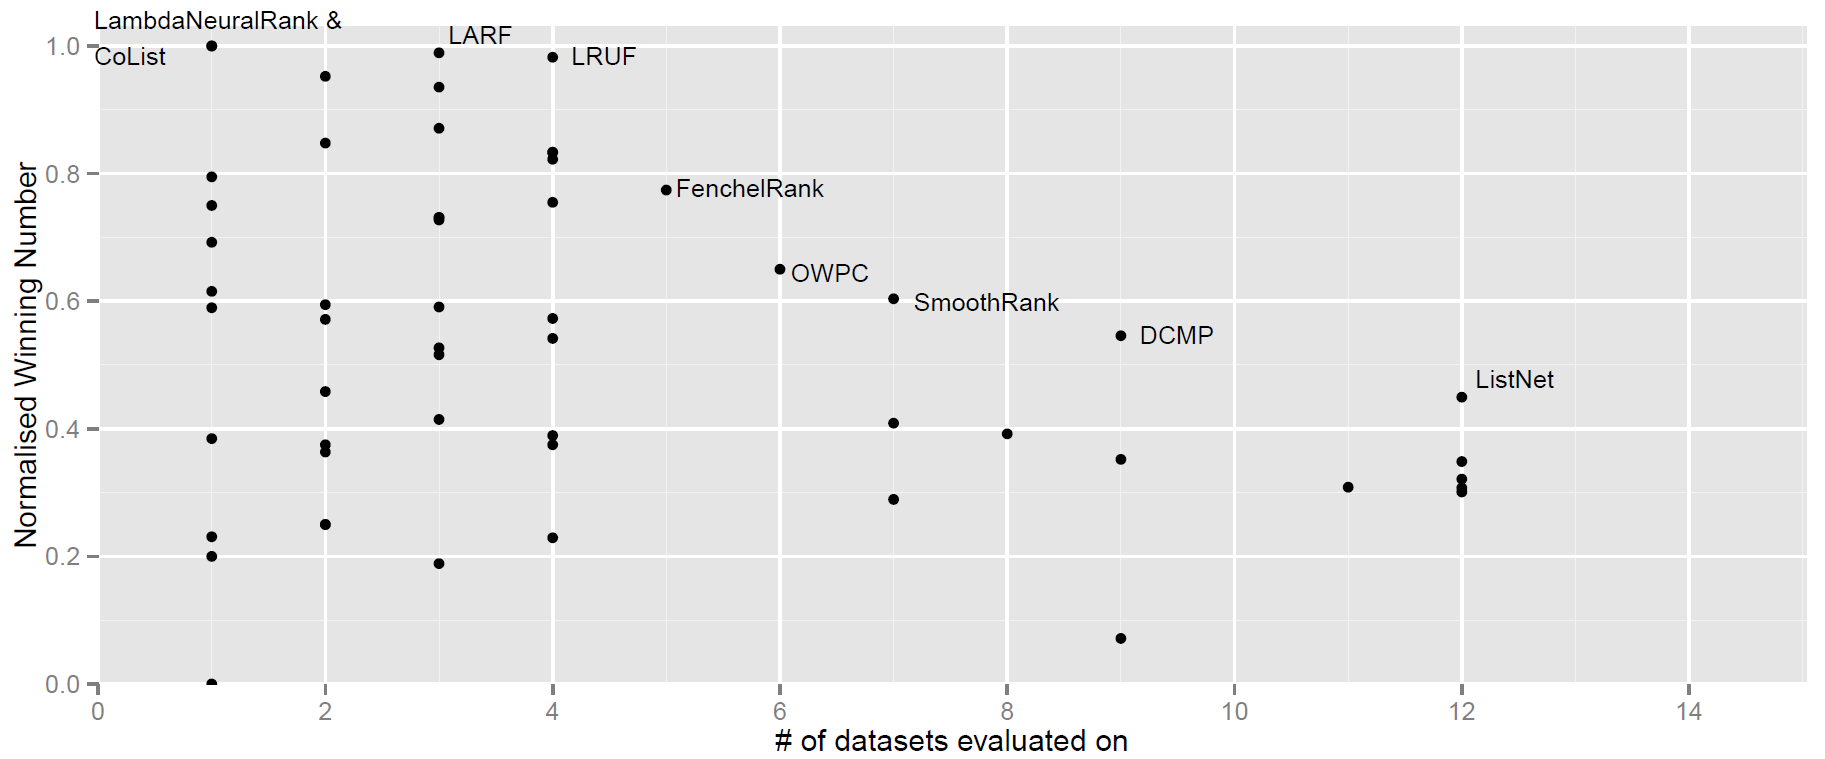
\includegraphics[scale=0.285]{gfx/ndcg3_winnum}
\caption{NDCG@3 comparison of Learning-to-Rank methods}
\label{fig:normalised_winning_number_ndcg3}
\end{figure}

LambdaNeuralRank and CoList both acquired a perfect Normalised Winning Number score of 1.0 by beating all other algorithms on one dataset, with LambdaNeuralRank winning on the AOL dataset and CoList winning on Yahoo Set 2. LARF and LRUF both scored very high scores of near 1.0 on three of the LETOR 3.0 datasets, which can be said to have a higher degree of certainty on the methods' performance because they are validated on three datasets which in addition are more relevant datasets than AOL and Yahoo Set 2 because there are more evaluation results available for the LETOR 3.0 datasets (see Table \ref{tab:ltr_methods_used}). FenchelRank, OWPC, SmoothRank, DCMP and ListNet are in that order increasingly lower in Normalised Winning Number, but increasingly higher in number of datasets that they are evaluated on, resulting in a higher degree of certainty on the accuracy of the algorithms.\\

LambdaNeuralRank, CoList, LARF, LRUF, OWPC and DCMP evaluation results are all based on one study, therefore are subjected to the risk of one overly optimistic study producing those results. FenchelRank evaluation result are based combined result from two studies, although those studies have overlap in authors. SmoothRank and ListNet have the most reliable evaluation result source, as they were official LETOR baseline runs.  

\subsection{NDCG@5}
Figure \ref{fig:normalised_winning_number_ndcg5} shows the performance of Learning-to-Rank methods for the NDCG@5 metric. Table \ref{tab:raw_data_norm_winnum_ndcg5} in Appendix \ref{app:norm_winnum_ndcg5} provides the raw Normalised Winning Number data for the Learning-to-Rank methods.\\

\begin{figure}[!h]
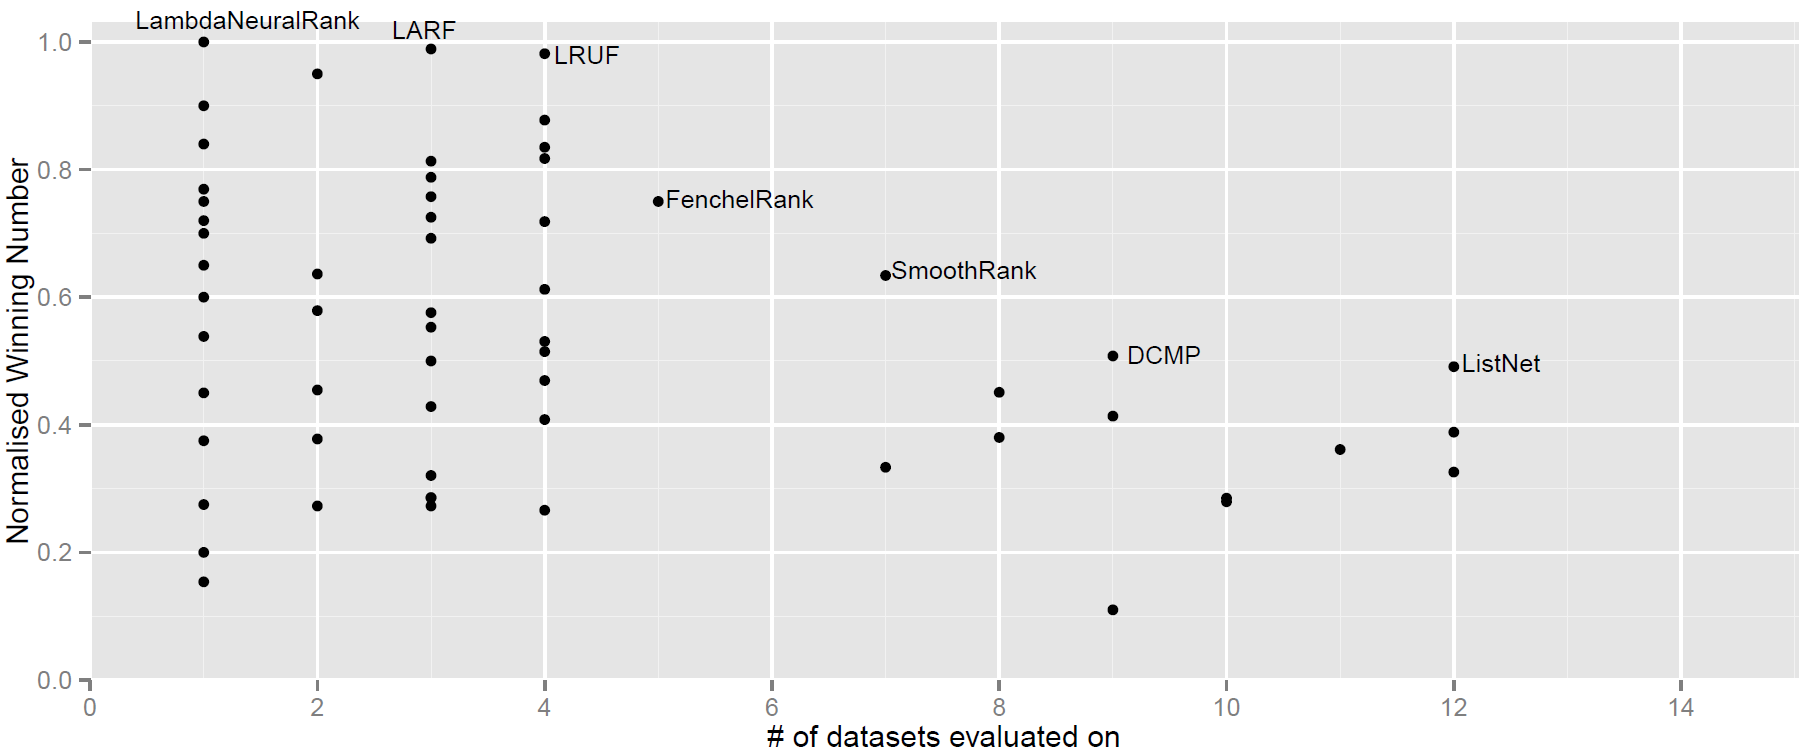
\includegraphics[scale=0.285]{gfx/ndcg5_winnum}
\caption{NDCG@5 comparison of Learning-to-Rank methods}
\label{fig:normalised_winning_number_ndcg5}
\end{figure}

LambdaNeuralRank again beat all other methods solely with results on the AOL dataset scoring a Normalised Winning Number of 1.0. LARF, LRUF, FenchelRank, SmoothRank, DCMP and ListNet are from left to right evaluated on an increasing number of datasets, but score decreasingly well in terms of Normalised Winning Number. These results are highly in agreement with the NDCG@3 comparison. The only modification compared to the NDCG@3 comparison being that OWPC did show to be a method for which there were no methods performing better on both axes in the NDCG@5 comparison, but not in the NDCG@3 comparison. Like in the NDCG@3 comparison, SmoothRank and ListNet can be regarded as most reliable results because the evaluation measurements for these methods are based on LETOR official baselines.

\subsection{NDCG@10}
Figure \ref{fig:normalised_winning_number_ndcg10} shows the performance of Learning-to-Rank methods for the NDCG@10 metric. Table \ref{tab:raw_data_norm_winnum_ndcg10} in Appendix \ref{app:norm_winnum_ndcg10} provides the raw Normalised Winning Number data for the Learning-to-Rank methods.\\

\begin{figure}[!h]
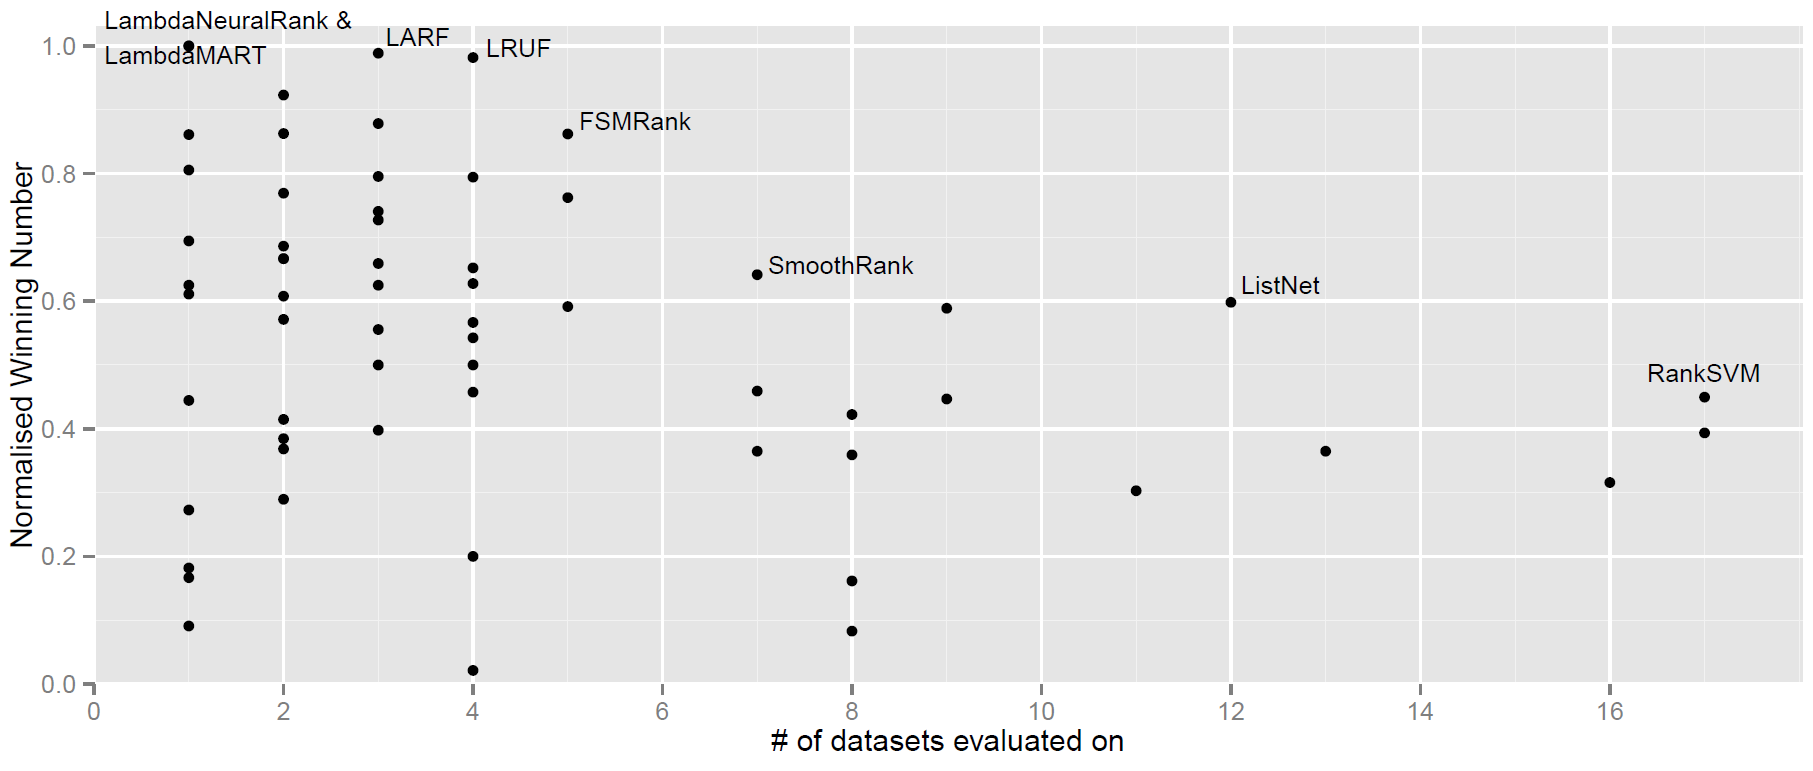
\includegraphics[scale=0.285]{gfx/ndcg10_winnum}
\caption{NDCG@10 comparison of Learning-to-Rank methods}
\label{fig:normalised_winning_number_ndcg10}
\end{figure}

LambdaMART and LambdaNeuralRank score a Normalised Winning Number of 1.0 on the NDCG@10 comparison. For LambdaNeuralRank these results are again based on AOL dataset measurements. LambdaMART showed the highest NDCG@10 performance for the MSLR-WEB10k dataset. The set of algorithms for which there is no other algorithm with both a higher Normalised Winning Number and number of datasets evaluated on is partly in agreement with those for the NDCG@3 and NDCG@5 comparisons: {LARF, LRUF, FSMRank, SmoothRank, ListNet, RankSVM}. SmoothRank and FSMRank were not present in this set for the NDCG@3 and NDCG@5 comparison, but were close by, as can be seen in Tables \ref{tab:raw_data_norm_winnum_ndcg3} and \ref{tab:raw_data_norm_winnum_ndcg5} in the Appendices. DCMP is not in the set in contrast with the NDCG@3 and NDCG@5 comparison.

\subsection{MAP}
Figure \ref{fig:normalised_winning_number_map} shows the performance of Learning-to-Rank methods for the MAP metric. Table \ref{tab:raw_data_norm_winnum_map} in Appendix \ref{app:norm_winnum_map} provides the raw Normalised Winning Number data for the Learning-to-Rank methods.\\

\begin{figure}[!h]
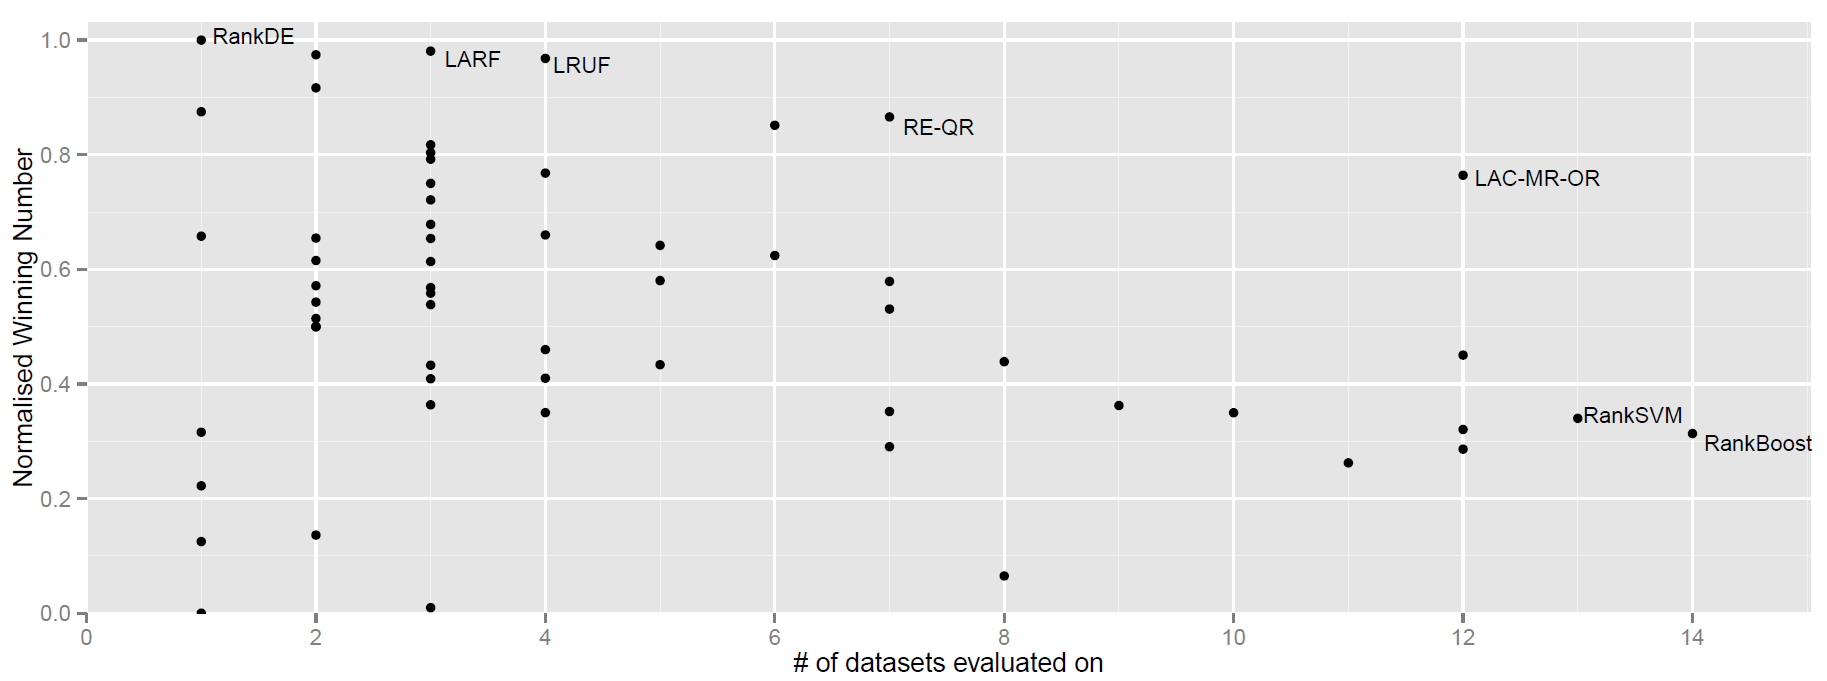
\includegraphics[scale=0.285]{gfx/map_winnum}
\caption{MAP comparison of Learning-to-Rank methods}
\label{fig:normalised_winning_number_map}
\end{figure}

Where comparisons on the NDCG metric at different cut-off points where highly in agreement in terms of the best performing algorithms, the comparison in terms of MAP shows different results. RankDE scores a Normalised Winning Number of 1.0 on one dataset, like LambdaNeuralRank did on for all NDCG-comparisons. In contrast to LambdaNeuralRank, RankDE achieved this highest score on the LETOR 2.0 TD2003, a dataset on which many methods are evaluated.\\

LARF and LRUF score very high Normalised Winning Number scores, but based on only relatively few datasets, just as in the NDCG comparisons. Notable is that SmoothRank and ListNet, which showed both high accuracy and high certainty on all NDCG comparisons, are not within the best performing methods in the MAP comparison. A deeper look in the raw data Tables \ref{tab:raw_data_norm_winnum_ndcg3} to \ref{tab:raw_data_norm_winnum_map} in Appendices \ref{app:norm_winnum_ndcg3} to \ref{app:norm_winnum_map} shows that LAC-MR-OR is evaluated on many more datasets for MAP compared to NDCG, which resulted in LAC-MR-OR obtaining equal certainty to ListNet with a higher Normalised Winning Number. SmoothRank performed a Normalised Winning Number of around 0.53 over 7 datasets, which is still good in both certainty and accuracy, but not among the top methods. RE-QR is one of the best performers in the MAP comparison with a reasonable amount of benchmark evaluations. No reported NDCG performance was found in the literature study for RE-QR. There is a lot of certainty on the accuracy of RankBoost and RankSVM as both models are evaluated on the majority of datasets included in the comparison for the MAP metric, but given their Normalised Winning Number it can said that both methods are not within the top performing Learning-to-Rank methods.

\subsection{Cross-metric}
Figure \ref{fig:normalised_winning_number_all} shows the Normalised Winning Number as function of Ideal Winning Number for the methods described in Table \ref{tab:ltr_methods_used}. Table \ref{tab:raw_data_norm_winnum_all} in Appendix \ref{app:norm_winnum_all} provide the raw data plotted in Figure \ref{fig:normalised_winning_number_all}.\\

\begin{figure}[!h]
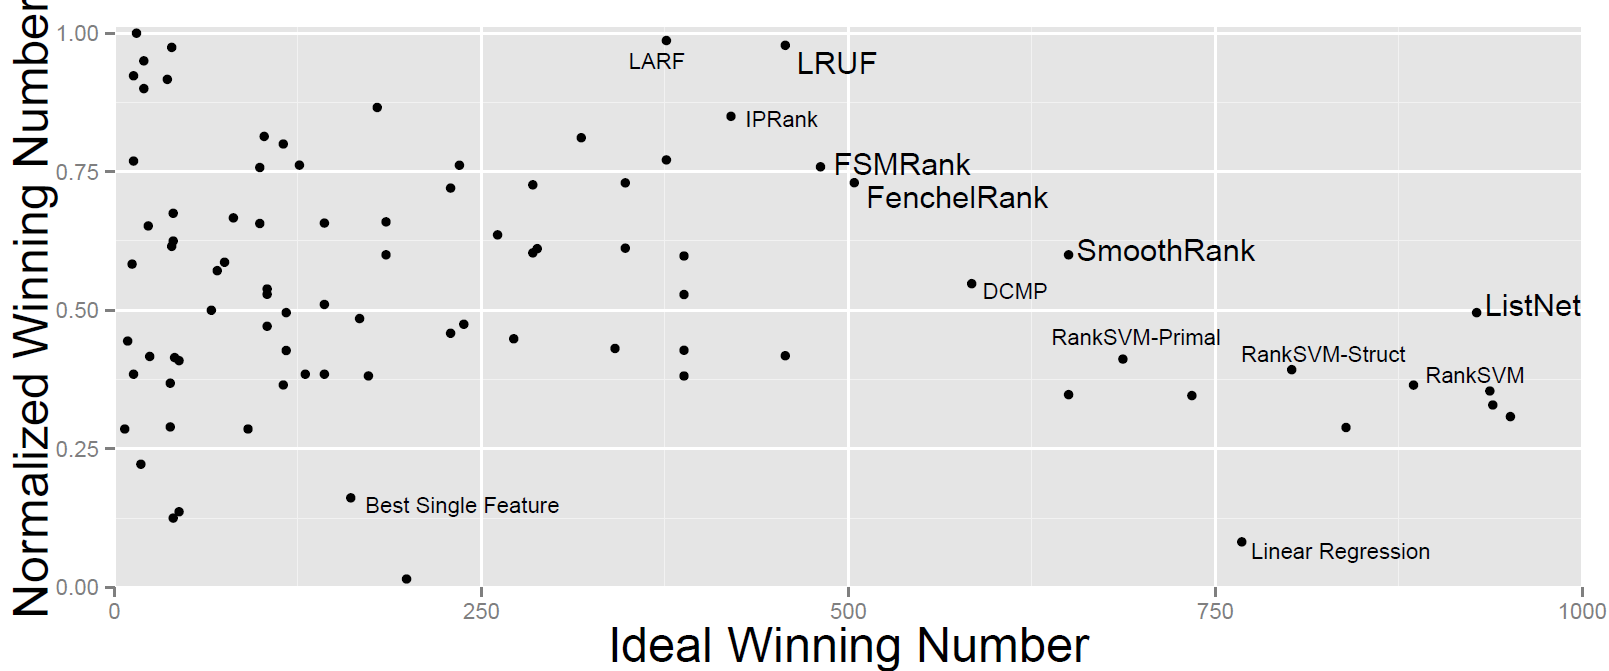
\includegraphics[scale=0.33]{gfx/combined_normalized_winnum}
\caption{Cross-benchmark comparison of Learning-to-Rank methods}
\label{fig:normalised_winning_number_all}
\end{figure}

The cross-metric comparison is based on the NDCG@3, NDCG@5, NDCG@10 and MAP comparisons combined, which justifies analysing the comparison more thoroughly. Figure \ref{fig:normalised_winning_number_all} labels the algorithms with no other algorithm having a higher value on both the horizontal axis and vertical axis, but also labels the algorithms with exactly one algorithm having a higher value on both axes with smaller font size. In addition, Linear Regression and the ranking method of simply sorting on the best single feature are labelled as baselines.\\

LRUF, FSMRank, FenchelRank, SmoothRank and ListNet showed to be the methods that have no other method superior to them in both Ideal Winning Number and Normalised Winning Number. LRUF is the only method that achieved this in all NDCG comparisons, the MAP comparison as well as the cross-metric comparison. With FenchelRank, FSMRank, SmoothRank and ListNet being among the top performing methods in all NDCG comparisons as well as in the cross-metric comparison, it can be concluded that the cross-metric results are highly defined by the NDCG performance as opposed to the MAP performance. This was to be expected, because the cross-metric comparison input data of three NDCG entries (@3, @5, and @10) enables it to have up to three times as many as many weight as the MAP comparison.\\

LARF, IPRank and DCMP and several variants of RankSVM performed very well on the cross-metric comparison, with all having only one method in its top right quadrant. LARF also performed among the top methods on the NDCG and MAP comparisons and DCMP was a top performer in a few of the NDCG comparisons.\\

C-CRF, DirectRank, FP-Rank, RankCSA, LambdaNeuralRank and VFLR all have near-perfect Normalised Winning Number measures, but have low Ideal Winning Number measures. Further evaluation runs of these methods on benchmark datasets that they are not yet evaluated on are desirable. The DirectRank paper \cite{Tan2013} shows that the method  is evaluated on more datasets than the number of datasets that we included evaluation results for in this meta-analysis. Some of the DirectRank measurements could not be used because measurements on some datasets were only available in graphical form and not in raw data.\\

LAC-MR-OR and RE-QR showed very good ranking accuracy in the MAP comparison on multiple datasets. Because LAC-MR-OR is only evaluated on two datasets for NDCG@10 and RE-QR is not evaluated for NDCG at all, LAC-MR-OR and RE-QR are not within the top performing methods in the cross-metric comparison. 

\section{Limitations}
In the Normalised Winning Number calculation the weight of each benchmark on the total score is determined by the number of evaluation measurements on this benchmark. By calculating it in this way, we implicitly make the assumption that the Learning-to-Rank methods are (approximately) distributed uniformly over the benchmarks, such that the average Learning-to-Rank method tested are approximately equally hard for each data set. It could be the case however that this assumption is false and that significantly more accurate Learning-to-Rank methods are evaluated on some datasets than on other datasets. \\

A second limitation is that the datasets on which Learning-to-Rank methods have been evaluated can not always be regarded a random choice. It might be the case that some researchers chose to publish results for exactly those benchmark datasets that showed the most positive results for their Learning-to-Rank method.\\

Another limitation lies in the meta-analysis methodology. Using evaluation results published by other researchers relies on the honesty of those researchers. Overly optimistic evaluation results published by other researchers do affect our Normalised Winning Number results. Limiting the meta-analysis to those studies that report comparable results on one of the baseline methods of a benchmark set reduces this limitation but does not solve it completely. By taking the Ideal Winning Number into account in Figure \ref{fig:normalised_winning_number_all} we further mitigate this limitation, as the Ideal Winning Number is loosely related with the number of studies that reported evaluation results for an algorithm.

\section{Conclusions}
We will now look back on our first research question using the knowledge gained with the cross-benchmark comparison.
\begin{description}
\item[RQ1] What are the best performing Learning-to-Rank algorithms in terms of accuracy on relevant benchmark datasets?\\
\end{description}
Although no closing arguments can be formulated on which Learning-to-Rank methods are most accurate, a lot of insight has been gained with the cross-benchmark comparison on which methods tend to perform better than others.\\

LRUF, FSMRank, FenchelRank, SmoothRank and ListNet were the Learning-to-Rank algorithms for which it holds that no other algorithm produced more accurate rankings with a higher degree of certainty of ranking accuracy. From left to right, the ranking accuracy of these methods decreases while the certainty of the ranking accuracy increases. For more definite conclusions on the relative performance of these five methods, more evaluation runs on are desirable for the methods on the left side on the list on benchmark datasets that these methods have not yet been evaluated on.\\


%
% The following two commands are all you need in the
% initial runs of your .tex file to
% produce the bibliography for the citations in your paper.
\bibliographystyle{abbrv}
\bibliography{sigproc}  % sigproc.bib is the name of the Bibliography in this case
% You must have a proper ".bib" file
%  and remember to run:
% latex bibtex latex latex
% to resolve all references
%
% ACM needs 'a single self-contained file'!
%
%APPENDICES are optional
%\balancecolumns
\appendix
\section{Raw Data for NDCG@3 Comparison}
\label{app:norm_winnum_NDCG3}

\begin{table}
\begin{tabular}{l|l|l}
Method & Normalised Winning Number & \# of datasets \\
\hline
AdaRank-MAP & 0.34862385 & 12 \\ 
AdaRank-NDCG & 0.30733945 & 12 \\ 
ApproxNDCG & 0.79487179 & 1 \\ 
BagBoo & 0.84782609 & 2 \\ 
BL-MART & 0.95238095 & 2 \\ 
BoltzRank-Pair & 0.83333333 & 4 \\ 
BoltzRank-Single & 0.75490196 & 4 \\ 
BT & 0.72727273 & 3 \\ 
CoList & 1.00000000 & 1 \\ 
DCMP & 0.54591837 & 9 \\ 
EnergyNDCG & 0.36363636 & 2 \\ 
FBPCRank & 0.41463415 & 3 \\ 
FenchelRank & 0.77419355 & 5 \\ 
FocusedBoost & 0.37500000 & 2 \\ 
FocusedNet & 0.45833333 & 2 \\ 
FocusedSVM & 0.25000000 & 2 \\ 
FRank & 0.30845771 & 11 \\ 
FSMRank & 0.83333333 & 4 \\ 
FSMSVM & 0.22916667 & 4 \\ 
GAS-E & 0.37500000 & 4 \\ 
GPRank & 0.87096774 & 3 \\ 
GroupCE & 0.73118280 & 3 \\ 
GroupMLE & 0.52688172 & 3 \\ 
IntervalRank & 0.58974359 & 1 \\ 
IPRank & 0.93548387 & 3 \\ 
KL-CRF & 0.59459459 & 2 \\ 
LambdaMART & 0.57142857 & 2 \\ 
LambdaNeuralRank & 1.00000000 & 1 \\ 
LambdaRank & 0.20000000 & 1 \\ 
LARF & 0.98924731 & 3 \\ 
Linear Regression & 0.07142857 & 9 \\ 
ListMLE & 0.00000000 & 1 \\ 
ListNet & 0.44954128 & 12 \\ 
ListReg & 0.73118280 & 3 \\ 
LRUF & 0.98230088 & 4 \\ 
MHR & 0.75000000 & 1 \\ 
NewLoss & 0.51612903 & 3 \\ 
OWPC & 0.65000000 & 6 \\ 
PERF-MAP & 0.38938053 & 4 \\ 
RankBoost & 0.32110092 & 12 \\ 
RankELM (pairwise) & 0.61538462 & 1 \\ 
RankELM (pointwise) & 0.69230769 & 1 \\ 
RankNet & 0.18867925 & 1 \\ 
RankSVM & 0.30097087 & 12 \\ 
RankSVM-Primal & 0.39204545 & 8 \\ 
RankSVM-Struct & 0.35204082 & 9 \\ 
REG-SHF-SDCG & 0.38461538 & 1 \\ 
Ridge Regression & 0.40880503 & 7 \\ 
RSRank & 0.57291667 & 4 \\ 
SmoothRank & 0.60377358 & 7 \\ 
SoftRank & 0.23076923 & 1 \\ 
SortNet & 0.25000000 & 2 \\ 
SparseRank & 0.82242991 & 4 \\ 
SVMMAP & 0.28930818 & 7 \\ 
TGRank & 0.54166667 & 4 \\ 
TM & 0.59090909 & 3 \\
\end{tabular}
\caption{Raw data of Normalised Winning Number comparison on NDCG@3}
\label{tab:raw_data_norm_winnum_NDCG3}
\end{table}

\section{Raw Data for NDCG@5 Comparison}
\label{app:norm_winnum_NDCG5}

\begin{table}
\begin{tabular}{l|l|l}
Method & Normalised Winning Number & \# of datasets \\
\hline
AdaRank-MAP & 0.3883929 & 12 \\ 
AdaRank-NDCG & 0.3258929 & 12 \\ 
ApproxNDCG & 0.7500000 & 1 \\ 
BagBoo & 0.8400000 & 1 \\ 
BL-MART & 0.7200000 & 1 \\ 
BoltzRank-Pair & 0.8349515 & 4 \\ 
BoltzRank-Single & 0.7184466 & 4 \\ 
BT & 0.7878788 & 3 \\ 
C-CRF & 0.9500000 & 2 \\ 
DCMP & 0.5078534 & 9 \\ 
EnergyNDCG & 0.3777778 & 2 \\ 
FBPCRank & 0.5529412 & 3 \\ 
FenchelRank & 0.7500000 & 5 \\ 
FocusedBoost & 0.4545455 & 2 \\ 
FocusedNet & 0.6363636 & 2 \\ 
FocusedSVM & 0.2727273 & 2 \\ 
FPRank & 0.9000000 & 1 \\ 
FRank & 0.2849462 & 10 \\ 
FSMRank & 0.8775510 & 4 \\ 
FSMSVM & 0.4081633 & 4 \\ 
GAS-E & 0.4693878 & 4 \\ 
GPRank & 0.7252747 & 3 \\ 
IntervalRank & 0.3750000 & 1 \\ 
IPRank & 0.8131868 & 3 \\ 
Kernel-PCA & 0.2857143 & 3 \\ 
KL-CRF & 0.5789474 & 2 \\ 
LambdaNeuralRank & 1.0000000 & 1 \\ 
LambdaRank & 0.2000000 & 1 \\ 
LARF & 0.9890110 & 3 \\ 
Linear Regression & 0.1099476 & 9 \\ 
ListNet & 0.4910714 & 12 \\ 
ListReg & 0.6923077 & 3 \\ 
LRUF & 0.9816514 & 4 \\ 
MHR & 0.6000000 & 1 \\ 
NewLoss & 0.4285714 & 3 \\ 
PERF-MAP & 0.2660550 & 4 \\ 
Q.D.KNN & 0.3205128 & 3 \\ 
RankAggNDCG & 0.5000000 & 3 \\ 
RankBoost & 0.2794118 & 10 \\ 
RankDE & 0.5384615 & 1 \\ 
RankELM (pairwise) & 0.6500000 & 1 \\ 
RankELM (pointwise) & 0.7000000 & 1 \\ 
RankNet & 0.2857143 & 3 \\ 
Rank-PMBGP & 0.7692308 & 1 \\ 
RankSVM & 0.3612565 & 11 \\ 
RankSVM-Primal & 0.4508671 & 8 \\ 
RankSVM-Struct & 0.4136126 & 9 \\ 
RCP & 0.5757576 & 3 \\ 
REG-SHF-SDCG & 0.4500000 & 1 \\ 
Ridge Regression & 0.3333333 & 7 \\ 
RSRank & 0.5306122 & 4 \\ 
SmoothRank & 0.6339869 & 7 \\ 
SoftRank & 0.2750000 & 1 \\ 
SortNet & 0.5147059 & 4 \\ 
SparseRank & 0.8173077 & 4 \\ 
SVD-RankBoost & 0.2727273 & 3 \\ 
SVMMAP & 0.3801170 & 8 \\ 
SwarmRank & 0.1538462 & 1 \\ 
TGRank & 0.6122449 & 4 \\ 
TM & 0.7575758 & 3 \\ 
\end{tabular}
\caption{Raw data of Normalised Winning Number comparison on NDCG@5}
\label{tab:raw_data_norm_winnum_NDCG5}
\end{table}

\section{Raw Data for NDCG@10 Comparison}
\label{app:norm_winnum_NDCG10}

\begin{table}
\begin{tabular}{l|l|l}
Method & Normalised Winning Number & \# of datasets \\
\hline
AdaRank-MAP & 0.36480687 & 13 \\ 
AdaRank-NDCG & 0.31578947 & 16 \\ 
ADMM & 0.44444444 & 1 \\ 
ApproxNDCG & 0.86111111 & 1 \\ 
Best Single Feature & 0.16149068 & 8 \\ 
CA & 0.65217391 & 4 \\ 
CoList & 0.16666667 & 1 \\ 
Consistent-RankCosine & 0.76923077 & 2 \\ 
DCMP & 0.58883249 & 9 \\ 
DirectRank & 0.92307692 & 2 \\ 
EnergyNDCG & 0.41463415 & 2 \\ 
FenchelRank & 0.76229508 & 5 \\ 
FocusedBoost & 0.68627451 & 2 \\ 
FocusedNet & 0.86274510 & 2 \\ 
FocusedSVM & 0.60784314 & 2 \\ 
FRank & 0.30288462 & 11 \\ 
FSMRank & 0.86206897 & 5 \\ 
FSMSVM & 0.54255319 & 4 \\ 
GAS-E & 0.45744681 & 4 \\ 
GP & 0.66666667 & 2 \\ 
GPRank & 0.65909091 & 3 \\ 
GRankRLS & 0.28947368 & 2 \\ 
GroupCE & 0.72727273 & 3 \\ 
GroupMLE & 0.62500000 & 3 \\ 
IPRank & 0.79545455 & 3 \\ 
LAC-MR-OR & 0.66666667 & 2 \\ 
LambdaMART & 1.00000000 & 1 \\ 
LambdaNeuralRank & 1.00000000 & 1 \\ 
LambdaRank & 0.57142857 & 2 \\ 
LARF & 0.98863636 & 3 \\ 
Linear Regression & 0.08287293 & 8 \\ 
ListMLE & 0.02127660 & 4 \\ 
ListNet & 0.59821429 & 12 \\ 
LRUF & 0.98181818 & 4 \\ 
MHR & 0.62500000 & 1 \\ 
NewLoss & 0.39772727 & 3 \\ 
PERF-MAP & 0.20000000 & 4 \\ 
Q.D.KNN & 0.50000000 & 3 \\ 
RandomForest & 0.42236025 & 8 \\ 
RankAggNDCG & 0.87837838 & 3 \\ 
RankBoost & 0.39357430 & 17 \\ 
RankDE & 0.18181818 & 1 \\ 
RankELM (pairwise) & 0.69444444 & 1 \\ 
RankELM (pointwise) & 0.80555556 & 1 \\ 
RankNet & 0.59154930 & 5 \\ 
Rank-PMBGP & 0.27272727 & 1 \\ 
RankRLS & 0.36842105 & 2 \\ 
RankSVM & 0.44957983 & 17 \\ 
RankSVM-Primal & 0.45911950 & 7 \\ 
RankSVM-Struct & 0.44670051 & 9 \\ 
RCP & 0.74074074 & 3 \\ 
Ridge Regression & 0.36477987 & 7 \\ 
RSRank & 0.62765957 & 4 \\ 
SmoothGrad & 0.38461538 & 2 \\ 
SmoothRank & 0.64150943 & 7 \\ 
SoftRank & 0.61111111 & 1 \\ 
SortNet & 0.56666667 & 4 \\ 
SparseRank & 0.79439252 & 4 \\ 
SVD-RankBoost & 0.55555556 & 3 \\ 
SVMMAP & 0.35911602 & 8 \\ 
SwarmRank & 0.09090909 & 1 \\ 
TGRank & 0.50000000 & 4 \\
\end{tabular}
\caption{Raw data of Normalised Winning Number comparison on NDCG@10}
\label{tab:raw_data_norm_winnum_NDCG10}
\end{table}

\section{Raw Data for MAP Comparison}
\label{app:norm_winnum_map}

\begin{table}
\begin{tabular}{l|l|l}
Method & Normalised Winning Number & \# of datasets \\
\hline
Method & Normalised Winning Number & \# of datasets \\ 
AdaRank-MAP & 0.320610687 & 12 \\ 
AdaRank-NDCG & 0.286259542 & 12 \\ 
ApproxAP & 0.500000000 & 2 \\ 
BagBoo & 0.654545455 & 2 \\ 
BL-MART & 0.803571429 & 3 \\ 
BoltzRank-Pair & 0.580419580 & 5 \\ 
BoltzRank-Single & 0.433566434 & 5 \\ 
BT & 0.750000000 & 3 \\ 
CCRank & 0.615384615 & 2 \\ 
FenchelRank & 0.641791045 & 5 \\ 
FRank & 0.262295082 & 11 \\ 
FSMRank & 0.578947368 & 7 \\ 
FSMSVM & 0.350000000 & 4 \\ 
GAS-E & 0.410000000 & 4 \\ 
GP & 0.500000000 & 2 \\ 
GPRank & 0.817307692 & 3 \\ 
GroupCE & 0.721153846 & 3 \\ 
GroupMLE & 0.653846154 & 3 \\ 
IntervalRank & 0.315789474 & 1 \\ 
IPRank & 0.851351351 & 6 \\ 
KeepRank & 0.538461538 & 3 \\ 
LAC-MR-OR & 0.764192140 & 12 \\ 
LambdaMART & 0.678571429 & 3 \\ 
LARF & 0.980769231 & 3 \\ 
Linear Regression & 0.065000000 & 8 \\ 
ListMLE & 0.009615385 & 3 \\ 
ListNet & 0.450381679 & 12 \\ 
ListReg & 0.432692308 & 3 \\ 
LRUF & 0.968000000 & 4 \\ 
MCP & 0.571428571 & 2 \\ 
MHR & 0.000000000 & 1 \\ 
MultiStageBoost & 0.136363636 & 2 \\ 
OWPC & 0.624113475 & 6 \\ 
PERF-MAP & 0.768000000 & 4 \\ 
PermuRank & 0.409090909 & 3 \\ 
Q.D.KNN & 0.558441558 & 3 \\ 
RandomForest & 0.438888889 & 8 \\ 
RankAggNDCG & 0.792207792 & 3 \\ 
RankBoost & 0.313432836 & 14 \\ 
RankCSA & 0.916666667 & 2 \\ 
RankDE & 1.000000000 & 1 \\ 
RankELM (pairwise) & 0.514285714 & 2 \\ 
RankELM (pointwise) & 0.542857143 & 2 \\ 
RankMGP & 0.222222222 & 1 \\ 
Rank-PMBGP & 0.875000000 & 1 \\ 
RankSVM & 0.340000000 & 13 \\ 
RankSVM-Primal & 0.351955307 & 7 \\ 
RankSVM-Struct & 0.362385321 & 9 \\ 
RCP & 0.363636364 & 3 \\ 
REF-SHF-SDCG & 0.657894737 & 1 \\ 
RE-QR & 0.865921788 & 7 \\ 
Ridge Regression & 0.290502793 & 7 \\ 
RSRank & 0.660000000 & 4 \\ 
SmoothRank & 0.530726257 & 7 \\ 
SortNet & 0.500000000 & 2 \\ 
SVD-RankBoost & 0.568181818 & 3 \\ 
SVMMAP & 0.349775785 & 10 \\ 
SwarmRank & 0.125000000 & 1 \\ 
TGRank & 0.460000000 & 4 \\ 
TM & 0.613636364 & 3 \\ 
VFLR & 0.974358974 & 2 \\
\end{tabular}
\caption{Raw data of Normalised Winning Number comparison on MAP}
\label{tab:raw_data_norm_winnum_map}
\end{table}

\section{Raw Data on Normalised Winning Number for cross-comparison}
\label{app:norm_winnum_all}

\begin{table}
\begin{tabular}{l|l|l|l}
Method & Winning Number & Ideal Winning Number & Normalized Winning Number \\
\hline
AdaRank-MAP & 332 & 937 & 0.35432231 \\ 
AdaRank-NDCG & 293 & 951 & 0.30809674 \\ 
ADMM & 4 & 9 & 0.44444444 \\ 
ApproxAP & 33 & 66 & 0.50000000 \\ 
ApproxNDCG & 92 & 115 & 0.80000000 \\ 
BagBoo & 96 & 126 & 0.76190476 \\ 
Best Single Feature & 26 & 161 & 0.16149068 \\ 
BL-MART & 83 & 102 & 0.81372549 \\ 
BoltzRank-Pair & 254 & 348 & 0.72988506 \\ 
BoltzRank-Single & 213 & 348 & 0.61206897 \\ 
BT & 75 & 99 & 0.75757576 \\ 
C-CRF & 19 & 20 & 0.95000000 \\ 
CA & 15 & 23 & 0.65217391 \\ 
CCRank & 24 & 39 & 0.61538462 \\ 
CoList & 2 & 7 & 0.28571429 \\ 
Consistent-RankCosine & 10 & 13 & 0.76923077 \\ 
DCMP & 320 & 584 & 0.54794521 \\ 
DirectRank & 12 & 13 & 0.92307692 \\ 
EnergyNDCG & 50 & 130 & 0.38461538 \\ 
FBPCRank & 81 & 167 & 0.48502994 \\ 
FenchelRank & 368 & 504 & 0.73015873 \\ 
FocusedBoost & 73 & 143 & 0.51048951 \\ 
FocusedNet & 94 & 143 & 0.65734266 \\ 
FocusedSVM & 55 & 143 & 0.38461538 \\ 
FP-Rank & 18 & 20 & 0.90000000 \\ 
FRank & 242 & 839 & 0.28843862 \\ 
FSMRank & 365 & 481 & 0.75883576 \\ 
FSM$^{SVM}$ & 148 & 388 & 0.38144330 \\ 
GAS-E & 166 & 388 & 0.42783505 \\ 
GP & 7 & 12 & 0.58333333 \\ 
GPRank & 290 & 376 & 0.77127660 \\ 
GRankRLS & 11 & 38 & 0.28947368 \\ 
GroupCE & 207 & 285 & 0.72631579 \\ 
GroupMLE & 172 & 285 & 0.60350877 \\ 
IntervalRank & 50 & 117 & 0.42735043 \\ 
IPRank & 357 & 420 & 0.85000000 \\ 
KeepRank & 56 & 104 & 0.53846154 \\ 
Kernel-PCA RankBoost & 26 &  91 & 0.28571429 \\ 
KL-CRF &  44 & 75 & 0.58666667 \\ 
LAC-MR-OR & 179 & 235  & 0.76170213 \\ 
LambdaMART & 54 & 81 & 0.66666667 \\ 
LambdaNeuralRank & 15 & 15 & 1.00000000 \\ 
LambdaRank & 10 & 24 & 0.41666667 \\ 
LARF & 371 & 376 & 0.98670213 \\ 
Linear Regression & 63 & 761  & 0.08278581 \\ 
ListMLE & 3 & 199 & 0.01507538 \\ 
ListNet & 460 & 928 & 0.49568966 \\ 
ListReg & 176 & 288 & 0.61111111 \\ 
LRUF & 447 & 457 & 0.97811816 \\ 
MCP & 40 & 70 & 0.57142857 \\ 
MHR & 17 & 41 & 0.41463415 \\ 
MultiStageBoost & 6  & 44 & 0.13636364 \\ 
NewLoss & 122 & 272 & 0.44852941 \\ 
OWPC & 166 & 261 & 0.63601533 \\ 
PERF-MAP & 191 & 457 & 0.41794311 \\ 
PermuRank & 18 & 44 & 0.40909091 \\ 
Q.D.KNN & 105 & 229 & 0.45851528 \\ 
RandomForest & 147 & 341 & 0.43108504 \\ 
Rank-PMBGP & 27 & 40 & 0.67500000 \\ 
RankAggNDCG & 165 & 229 & 0.72052402 \\ 
RankBoost & 309 & 939 & 0.32907348 \\ 
RankCSA & 33 & 36 & 0.91666667 \\ 
RankDE & 25 & 40 & 0.62500000 \\ 
RankELM (pairwise) & 111 & 185 & 0.60000000 \\ 
RankELM (pointwise) & 122 & 185 & 0.65945946 \\ 
RankMGP & 4 & 18 & 0.22222222 \\ 
RankNet & 66 & 173 & 0.38150289 \\ 
RankRLS & 14 & 38 & 0.36842105 \\ 
RankSVM & 323 & 885 & 0.36497175 \\ 
RankSVM-Primal & 283 & 687 & 0.41193595 \\ 
RankSVM-Struct & 315 & 793 & 0.39276808 \\ 
RCP & 55 & 104 & 0.52884615 \\ 
RE-QR & 155 & 179 & 0.86592179 \\ 
REG-SHF-SDCG & 58 & 117 & 0.49572650 \\ 
Ridge Regression & 226 & 650 & 0.34769231 \\ 
RSRank & 232 & 388 & 0.59793814 \\ 
SmoothGrad & 5 & 13 & 0.38461538 \\ 
SmoothRank & 390 & 650 & 0.60000000 \\ 
SoftRank & 42 & 115 & 0.36521739 \\ 
SortNet & 113 & 238 & 0.47478992 \\ 
SparseRank & 258 & 318 & 0.81132075 \\ 
SVD-RankBoost & 49 & 104 & 0.47115385 \\ 
SVM$^{MAP}$ & 254 & 734 & 0.34604905 \\ 
SwarmRank & 5 & 40 & 0.12500000 \\ 
TGRank & 205 & 388 & 0.52835052 \\ 
TM & 65 & 99 & 0.65656566 \\ 
VFLR & 38 & 39 & 0.97435897 \\
\end{tabular}
\caption{Raw data of Normalised Winning Number comparison cross-metric}
\label{tab:raw_data_norm_winnum_all}
\end{table}

\end{document}
